\section{Spring models validation}
\label{sec:ModelValidation}

In order to validate the two modeling approaches, an experiment setup has been constructed as shown Figure~\ref{fig:Spring_torque_exp_setup}. The FourByThree 50 Nm SEA (for more details, see Section \ref{sec:SEAdesign}) is used and fixed on an adjustable base, so that the inclination of the actuator can be changed and the effects of gravity can be accounted for. An external force/torque sensor is mounted between the spring coupling and the link lever, which measures the output torque with a 125 Hz sampling frequency in order to validate the results.

%%%%%%%%%%%%%%%%%%%%     Figure: testbed      %%%%%%%%%%%%%%%%%%%%%%%%
\begin{figure}[htb]
\centering
\advance\leftskip 1.5cm
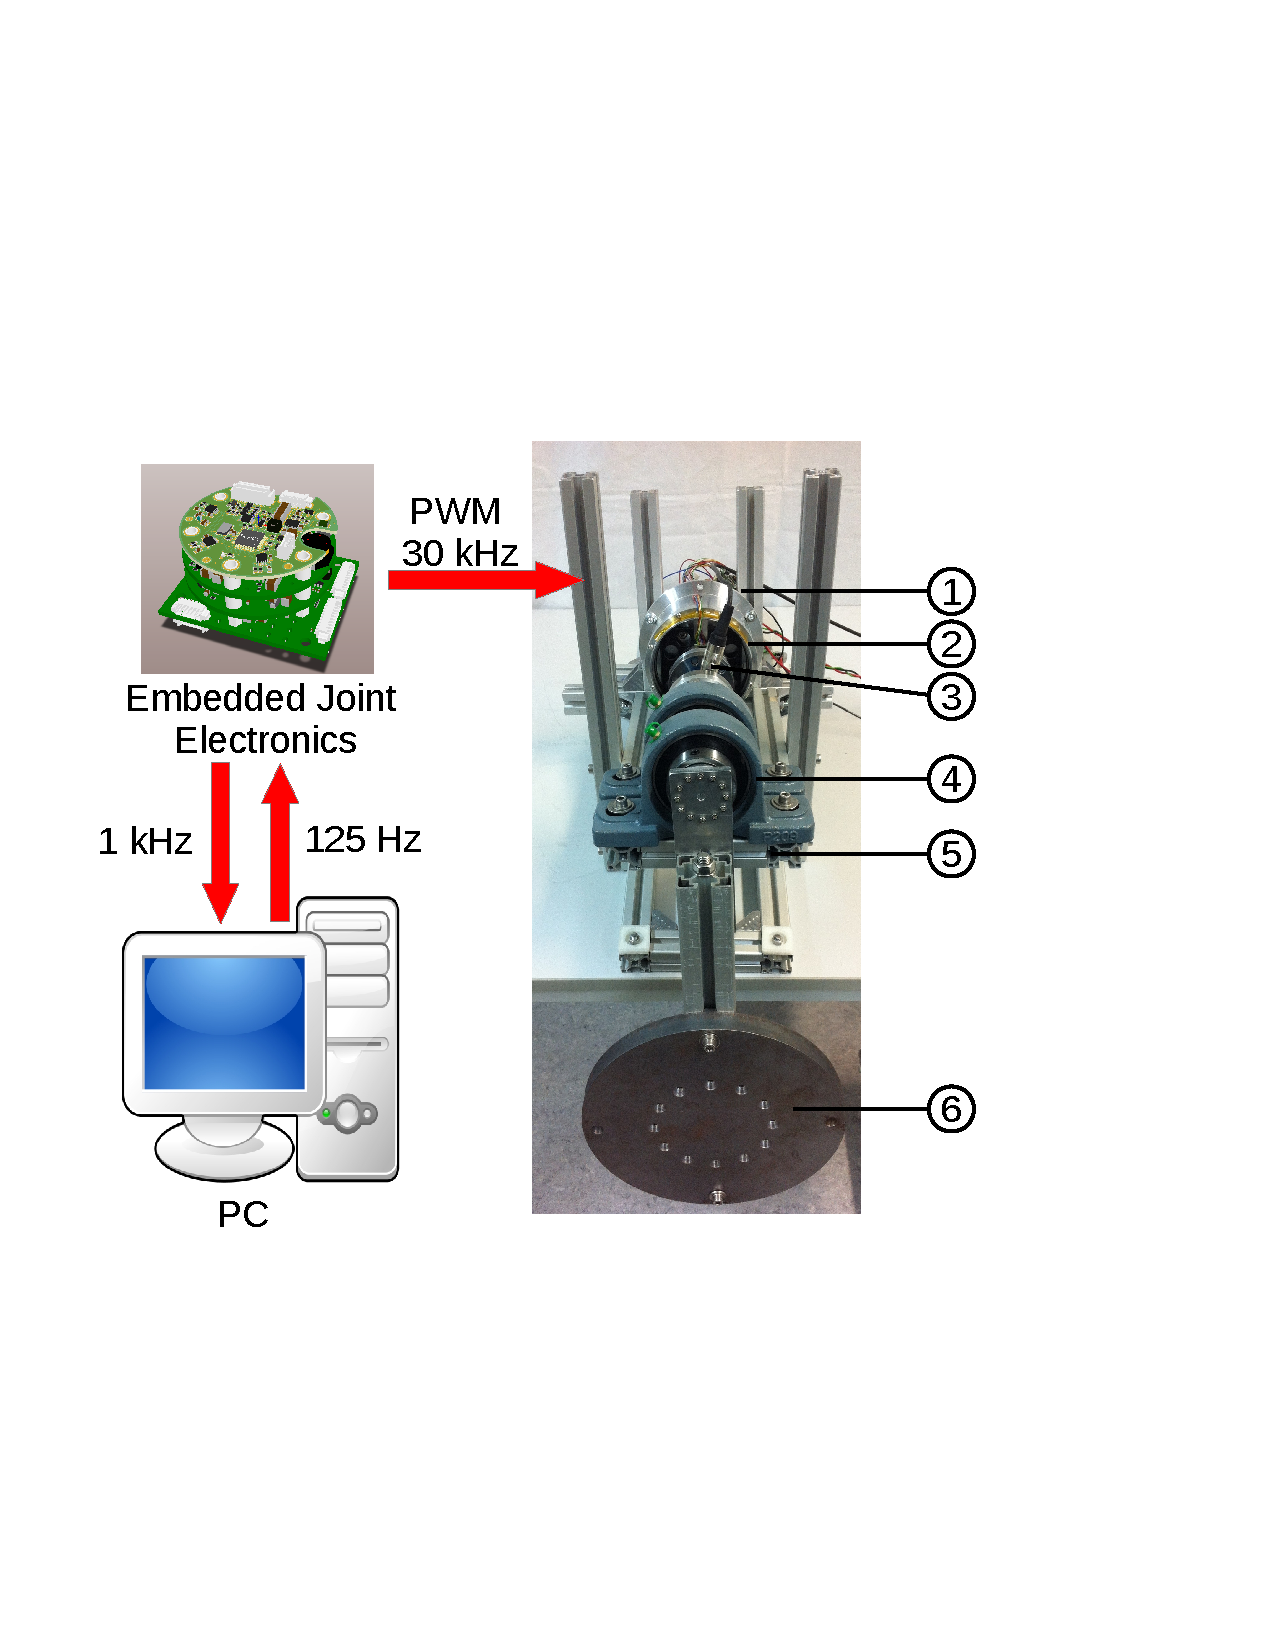
\includegraphics[clip, trim=0.5cm 7cm 0.5cm 7.5cm,width=0.88\columnwidth]{./images/4by3_springmodel_testbed.pdf} 
 \caption{Experimental setup used for spring modeling and torque control: 1) actuator; 2) spring coupling; 3) external force/torque sensor; 4) brake; 5) adjustable base; 6) load.}
 \label{fig:Spring_torque_exp_setup}
\end{figure}
%%%%%%%%%%%%%%%%%%%%%%%%%%%%%%%%%%%%%%%%%%%%%%%%%%%%%%%%%%%%%%%%%%%%%%%

The models need to be trained first and then be used in the validation phase by estimating the output torque given measured variables. In the training procedure, the inclination angle of the actuator base is set to 0 degree and the training data is gathered by controlling the load to rotate in the range of approx. $\pm170$ degrees with position control smoothly in a very low speed. %Since the load velocity and acceleration are approaching to zero, the velocity related dynamic effects can be neglected.  %Therefore, the nonlinearity of the spring coupling and the static friction are modelled in this experiment. 
The position of the load at the link lever is changed in each train test and the actuator torque $\tau$, deflection $\delta$, first derivative of deflection $\delta^{\prime}$ and velocity $v$ are measured as the training inputs. The spring deflection is extracted from two absolute encoders, the first derivative of deflection $\delta^{\prime}$ is calculated from the change of the deflection and the time used in a control cycle and the velocity $v$ is acquired from the position sensor. 

In the validation phase, the same load is fixed at random selected position on the lever arm and the inclination angle of the base is set to 37.8 degree. %Therefore, the data which gathered from testing experiment is different to the training data.
Based on the trained DGMM and neural network models, the actuator torque $\tau$ can be estimated by both methods respectively. Figure \ref{fig:springmodelcomparison} shows the comparison results between the trained DGMM model $P[\tau,\delta,\delta^{\prime},v]$, the neural network model, and the linear regression model.

%%%%%%%%%%%%%%%%%%%%  Figure: model comparison %%%%%%%%%%%%%%%%%%%%%%%%
\begin{figure}[htb]
\centering
\advance\leftskip-1.2cm
%\hspace*{-1.5in}
%\vspace*{-1.1 cm}
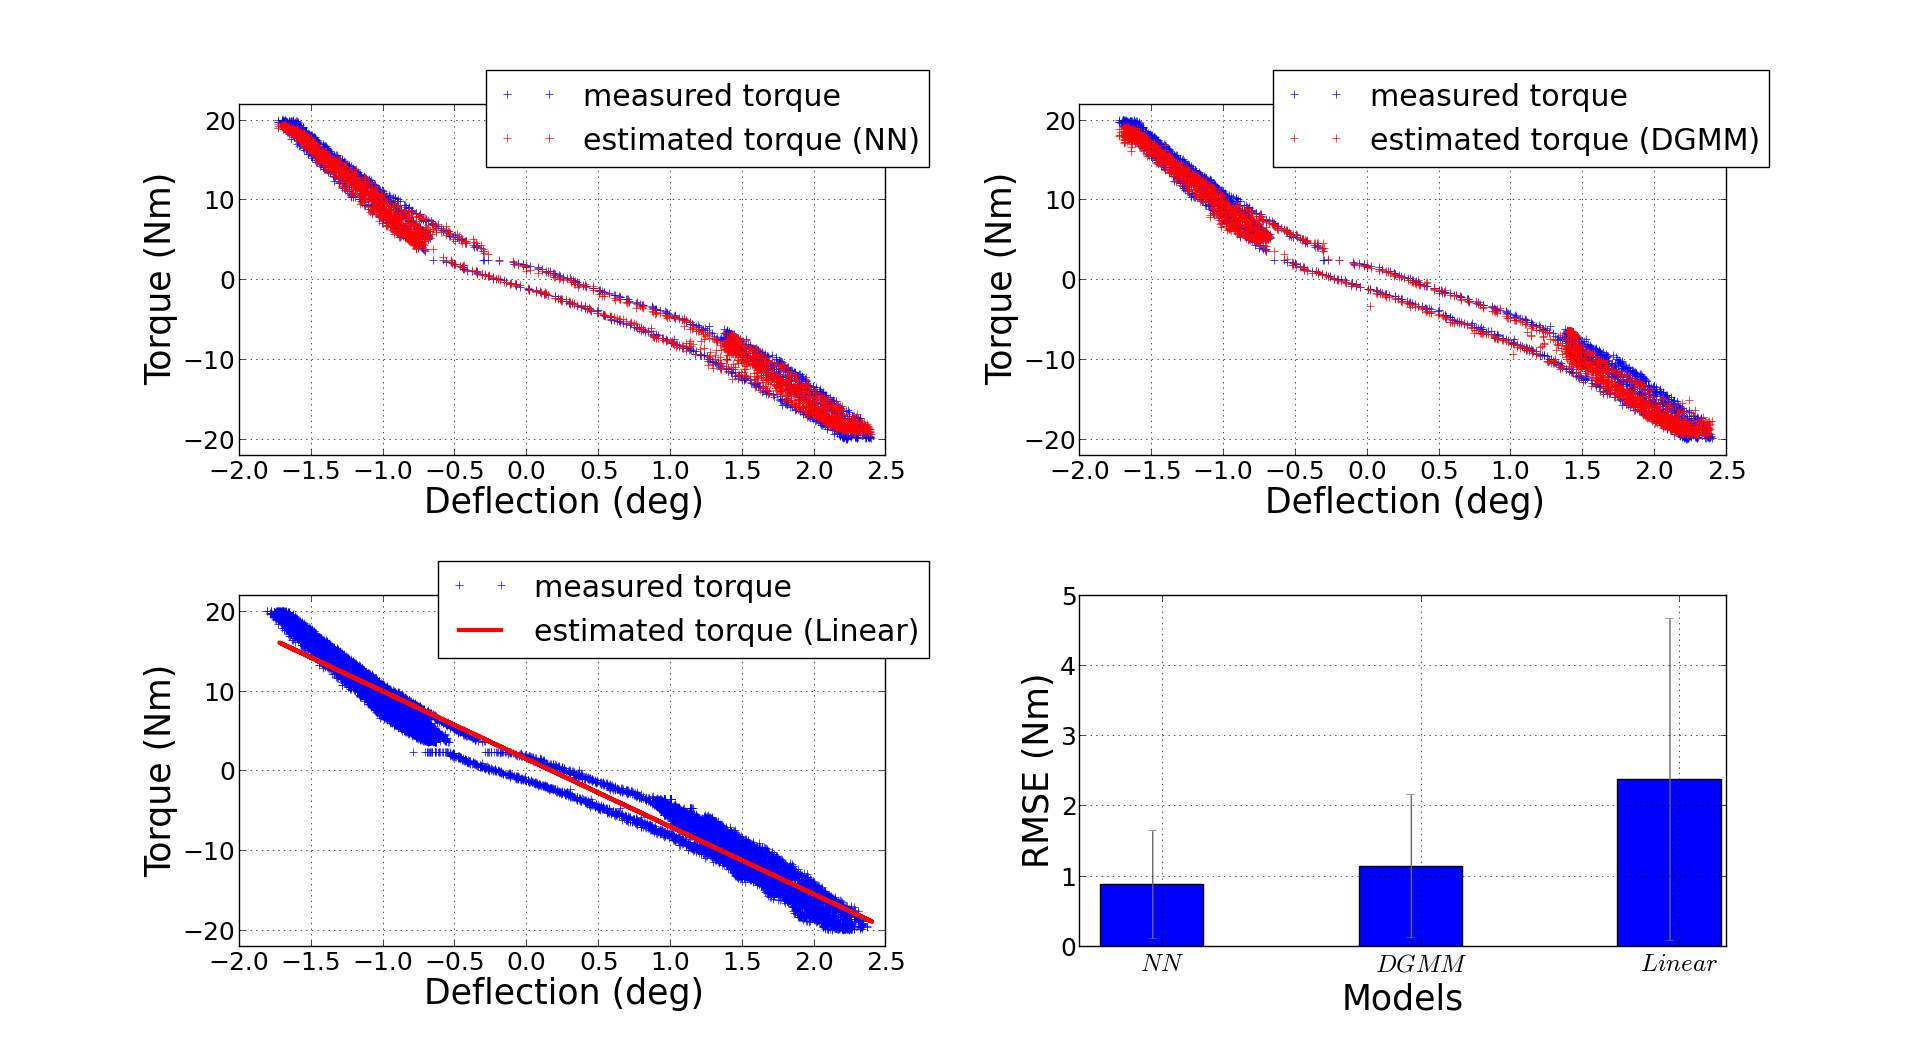
\includegraphics[width=1.22\columnwidth]{./images/4by3_model_comparison_new.png}
 \caption{\textit{Upper left:} measured torque-deflection curve (blue crosses) and estimated torque with neural network model (red crosses). \textit{Upper right:} measured torque-deflection curves (blue crosses) and estimated torque with DGMM model (red crosses), \textit{lower left:} measured torque-deflection curve (blue crosses) and corresponding fitted linear line (red line), \textit{lower right:} root mean square errors (blue bars) and normalized standard deviations (black line) of the three models in torque estimation.}
 \label{fig:springmodelcomparison}
\end{figure}
%%%%%%%%%%%%%%%%%%%%%%%%%%%%%%%%%%%%%%%%%%%%%%%%%%%%%%%%%%%%%%%%%%%%%%%

As can be seen from the upper left and upper right plots, both DGMM and neural network models are able to predict the output torque given the measured variables with high accuracy. In contrast, the fitted linear regression function has problems to represent the torque-deflection curve (see lower left plot). The RMSE between the estimated torque and measured torque is calculated for each model, as the lower right plot shows; the DGMM and neural network models present a comparable performances and have a large advantage compared to the linear model.



